\section{Introducci\'on al problema}
\subsection{Conjunto Independiente Dominante M\'inimo (CIDM)}

Sea $G = (V, E)$ un grafo simple. Un conjunto $D \subseteq V$ es un \emph{conjunto dominante} de $G$ si todo v\'ertice de $G$ est\'a en $D$ o bien tiene al menos un vecino que est\'a en $D$. 

Por otro lado, un conjunto $I \subseteq V$ es un \emph{conjunto independiente} de $G$ si no existe ning\'un eje de $E$ entre dos v\'ertices de $I$. 

Definimos entonces un \emph{conjunto independiente dominante} de $G$ como un conjunto independiente que a su vez es un conjunto dominante del grafo $G$.\\

El problema de Conjunto Independiente Dominante M\'inimo (CIDM) consiste en hallar un conjunto independiente dominante de $G$ con m\'inima cardinalidad.

\subsection{Paralelismo con ``El se\~nor de los caballos''}\label{caballitos}

El problema ``\emph{El se\~nor de los caballos}'' es similar al problema de encontrar un \emph{Conjunto Independiente Dominante M\'inimo} considerando solamente \textcolor{red}{al tablero inicial como vacío (?)} y una familia específica de grafos. Esta es la familia de grafos donde cada nodo modela un casillero de un tablero de ajedrez y sólo existe un eje entre dos nodos $v_1$ y $v_2$ si el movimiento desde $v_1$ a $v_2$ o \textit{viceversa} es un movimiento permitido para la pieza de un caballo.\\

  \begin{figure}[h!]
   \begin{center}
 	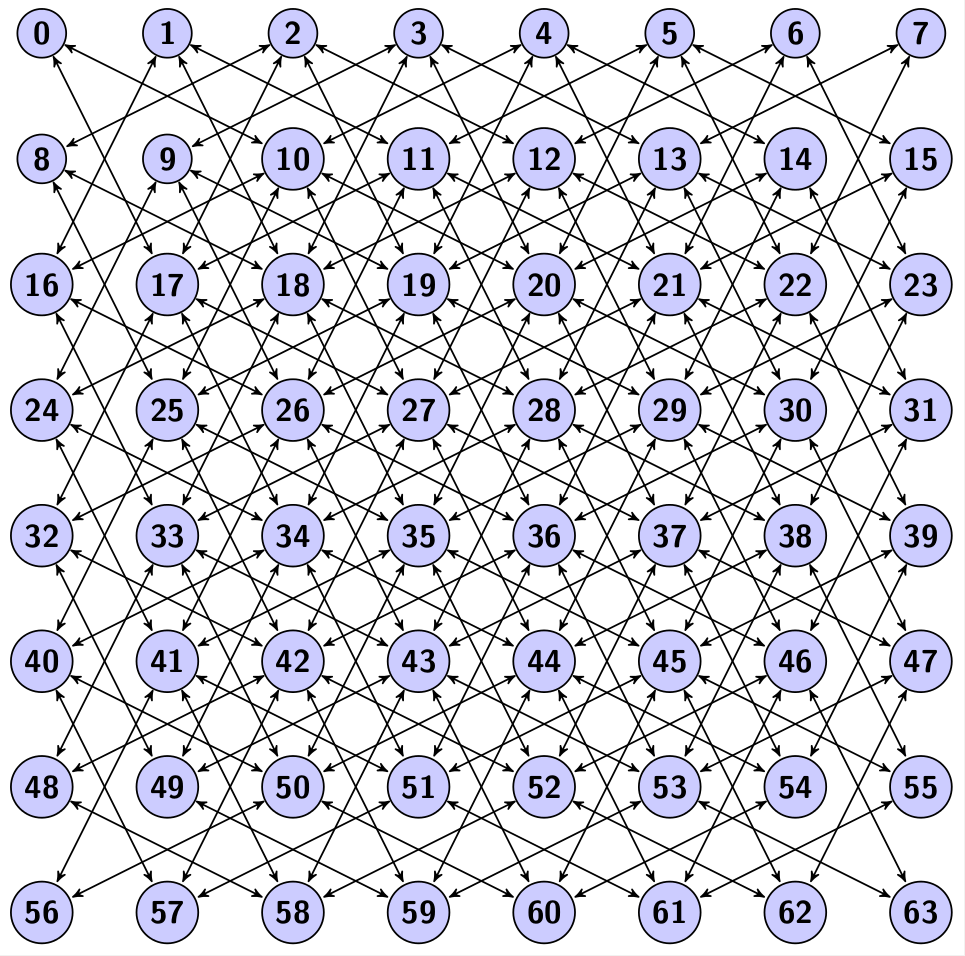
\includegraphics[scale=0.4]{imagenes/tablero8x8.png}
% 	\caption{}
	\label{GrafoCompleto}
   \end{center}
 \end{figure}

\textcolor{red}{Insertar imagen del grafo tablero}\\
\textcolor{blue}{Insertada, espero que les guste}\\

La relación con nuestro problema es la siguiente:
\begin{itemize}
	\item ``El se\~nor de los caballos'' busca un conjunto dominante, dado que intenta ocupar el tablero, y para ello requiere que o bien cada casillero tenga un caballo, o bien que cada casillero sea amenazado por un caballo.
	\item ``El se\~nor de los caballos'' busca un conjunto m\'inimo, es decir, que utilice la menor cantidad de caballos posibles.
	\item ``El se\~nor de los caballos'' \textbf{NO} busca un conjunto independiente, dado que si fuese necesario, un caballo puede ubicarse en un casillero que estuviese siendo amenazado por otro caballo.
	
\end{itemize}
%\newpage
\subsection{Todo conjunto independiente maximal es un conjunto dominante}

 Sea $G = (V, E)$ un grafo simple, un \emph{conjunto independiente} de $I \subseteq V$ se dice \emph{maximal} si no existe otro conjunto independiente $J \subseteq V$ tal que $I \subset J$, es decir que $I$ est\'a incluido estrictamente en $J$. \\
 
 Todo conjunto independiente maximal es un \emph{conjunto dominante}.
 
\subsubsection*{Demostraci\'on}

Sean $G = (V, E)$ grafo simple, $I \subseteq V$ \emph{conjunto independiente maximal}.\\

Quiero ver que $I$ es un \emph{conjunto dominante}: 

Lo que es equivalente a probar que $(\forall $ $nodo$ $ v \in V)$ $((v \in I) \vee (\exists $ $nodo$ $ w \in adyacentes(v), w \in I))$\\

\bigskip
Supongo por el absurdo que: 
$(\exists $ $nodo$ $ v \in V)$ $tq$ $((v\notin I)\wedge(\forall $ $nodo$ $w \in $ $adyacentes(v), w\notin I))$\\

Considero a $adyacentes(I)$ como el conjunto que se obtiene de concatenar todos los vecinos de cada elemento de $I$. Por lo tanto, es equivalente decir $(\forall $ $nodo$ $w \in $ $adyacentes(v), w\notin I)$ y decir $( v \notin adyacentes(I))$.\\

$\Rightarrow v\notin I \wedge v \notin adyacentes(I)$ 

$\Rightarrow \exists$ conjunto independiente $J$: $J\subseteq V$ tq $J=I+\{v\}$

$J$ es independiente porque $I$ lo era y al agregarle el nodo $v$ se mantiene esta propiedad ya que $v$ no pertenec\'ia a $I$ y adem\'as no estaba conectado a ning\'un nodo del conjunto $I$.

$\Rightarrow \exists J$ conjunto independiente tq $I \subset J$. \textbf{Absurdo!}($I$ era un conjunto Independiente Maximal)\\

El absurdo provino de suponer que $I$ era un conjunto independiente maximal, pero no dominante. Por lo tanto, $I$ debe ser un conjunto dominante.







%Dado que el conjunto $I$ es independiente, $\nexists $ $eje$ $ e=(n_1,n_2) \in E$ $tq$ $(n_1 \in I \wedge n_2 \in I)$\\

%Como $I$ es maximal, \textcolor{red}{No estoy segura de que esto valga (creo que ni lo entendi):} no existe ning\'un v\'ertice w de V que no pertenezca a I, tal que w no sea adyacente a alguno de I.\\


%Entonces:
%\begin{itemize}
%\item si E = $\emptyset$, I = V y por lo tanto cada elemento de v pertenece a I trivialmente
%\item si E $\neq$ $\emptyset$, todos los v\'ertices v $in$ V que no pertenezcan a I, no lo hacen porque ya existe w $in$ I que verifica que el eje (v,w) $in$ E. Luego, cada u v\'ertice de V o bien pertenece a I, o bien es adyacente a alg\'un elemento de I. Por lo tanto I es un conjunto dominante.
%\end{itemize}
\textcolor{blue}{se fijan que onda?}
%\textcolor{red}{Demostracion magica negra turbia}

\subsection{Situaciones de la vida real}

Situaciones de la vida real que puedan modelarse utilizando CIDM:

\begin{itemize}
	\item \textbf{Ubicación de estudiantes al momento de rendir un examen:} Encontrar la mejor manera de ubicar a todos los estudiantes en el aula, tal que ninguno esté suficientemente cerca de otro como para copiarse, pero tal que entre la mayor cantidad de estudiantes posibles. Esta situación es lo mismo que modelar el aula como un grafo donde cada asiento es un nodo y cada asiento es adyacente a los asientos que estan a sus costados (en todas las direcciones); luego buscar el \emph{CIDM} de dicho grafo.
	
	\item \textbf{Ubicación de servicios en ciudades:} Para minimizar costos, es probable que si se quiere situar centros de servicios (cualesquiera sean estos: hospitales, estaciones de servicio, distribuidoras, etc), se los situe de manera tal que tengan amplia cobertura, pero sin situar demasiados centros, es decir, situando la mínima cantidad. Tampoco se querría que un centro cubra la misma zona que otro centro. Si se modela a la ciudad, tomando cada zona (arbitraria, como barrios, o manzanas, o conjunto de manzana) como un nodo, en los que cada nodo es adyacente al nodo que representa la zona vecina, entonces el problema de situar estos centros minimizando costos, es igual a encontrar un \emph{CIDM} en el grafo mencionado.
\end{itemize}
